\documentclass{article}
\usepackage[utf8]{inputenc}

\title{Machine Learning, Sentence Trees}
\author{Bartłomiej Szymański}
\date{23-24 March 2019}

\usepackage{natbib}
\usepackage{graphicx}
\usepackage{hyperref}

\begin{document}

\maketitle

\section{Tokenization of sentences, words}
The dataset that is being provided to us contains multiple sentences. NLTK library for Python allows to tokenize\cite{Tokenization} the text into individual sentences with any given delimiters, and then each of the sentences into actual words. The order of operation in this case is important, because it allows to create multidimensional arrays where each sentence would be represented by an array stored in an array of sentences.\\ \\
Consider a set of sentences like:
\begin{quote}
This thing seemed to overpower and astonish the little dark-brown dog, and wounded him to the heart. He sank down in despair at the child's feet. When the blow was repeated, together with an admonition in childish sentences, he turned over upon his back, and held his paws in a peculiar manner. At the same time with his ears and his eyes he offered a small prayer to the child.
\end{quote}
The desired form of this sentence after applying Sentence Tokenization and then Word Tokenization is:
\begin{verbatim}
[
['This', 'thing', 'seemed', 'to', 'overpower', 'and', 'astonish', 
'the', 'little', 'dark-brown', 'dog', ',', 'and', 'wounded', 
'him', 'to', 'the', 'heart', '.'],
['He', 'sank', 'down', 'in', 'despair', 'at', 'the', "child's", 
'feet', '.'],
['When', 'the', 'blow', 'was', 'repeated', ',', 'together', 
'with', 'an', 'admonition', 'in', 'childish', 'sentences', ',', 
'he', 'turned', 'over', 'upon', 'his', 'back', ',', 'and', 'held', 
'his', 'paws', 'in', 'a', 'peculiar', 'manner', '.'],
['At', 'the', 'same', 'time', 'with', 'his', 'ears', 'and', 'his', 
'eyes', 'he', 'offered', 'a', 'small', 'prayer', 'to', 'the', 
'child', '.']
]
\end{verbatim}
You can achieve this form by using the following code from the NLTK library\cite{Demo of TweetTokenizer}:
\begin{verbatim}
    from nltk.tokenize import TweetTokenizer, sent_tokenize
    tokenizer_words = TweetTokenizer()
    tokens_sentences = [tokenizer_words.tokenize(t) for t in
    nltk.sent_tokenize(input_text)]
    print(tokens_sentences)
\end{verbatim}
To further optimize the list of sentences it is possible to remove punctuation from each of those sentences. Note that by this you might remove some context from the sentences that might become a useful feature in the feature space for Machine Learning.
\section{Exploring Sentence Trees}
To simplify this concept for the sake of our assignment, each sentence in any language can be deconstructed into a tree. To begin creating a Sentence Tree, it is necessary to assign PoS (Parts-of-Speech)\cite{POS} labels to every word in a given sentence. 
\subsection{Simple PoS Trees}
In NLTK, this can be done using this code.
\begin{verbatim}
sentences = [nltk.pos_tag(sent) for sent in sentences]
\end{verbatim}
Where sentences is an array of tokenized sentences, just like in the first section of this document. The output of this operation for a sentence
\begin{verbatim}
    The blogger taught the reader to chunk.
\end{verbatim}
becomes:
\begin{verbatim}
    [('The', 'DT'),
      ('blogger', 'NN'),
      ('taught', 'VBD'),
      ('the', 'DT'),
      ('reader', 'NN'),
      ('to', 'TO'),
      ('chunk', 'VB'),
      ('.', '.')]
\end{verbatim}
Description of all the labels NLTK can return is located here\cite{POS labels}. \\
In this case, the tree of this sentence looks like follows:
\begin{figure}[htb!]
    \centering
    
\includegraphics[width=\textwidth]{nickcdryanblog2.png}
    \caption{PoS labeled tree}
\end{figure}\\
This is a very basic tree. It does not give much information on dependencies between words, but is big enough to construct a basic feature space as long as you apply Chunking. Chunking is the process of grouping words together to provide us relevant blocks of information when it comes to sentences. \\ \\
The project that we've picked consists extracts PRP/PRP\$s from the sentences (prepositions, such as "He" or "his") and chunks of NNPs/NNPSs (Proper Nouns and Proper Nouns in Plural respectively, for example "Manchester United" or "Americans"). \\ \\
The easiest way to create chunks of NNPs and NNPSs is to connect cases when NNPs and NNPSs show up one after another, keeping in mind that punctuation does break the NNP blocks.
Consider the 158th entry of the dataset:
\begin{quote}
    On 17 June 2005, after 12 years at Birmingham, Bennett transferred to Leeds United who already had Scottish international goalkeeper Neil Sullivan as first-choice goalkeeper. Despite playing the pre-season friendlies, he was limited to four league appearances during the 2005-06 season, obtained deputising for the injured Sullivan.
\end{quote}
Though Birmingham and Benett are words that are next to one another, there is a comma between those two words, making them separate chunks of NNPs. Leeds United and Neil Sullivan will both be two-word long chunks of NNPs. \\ \\
The most simple feature space that can be extracted from this entry for this project would contain the following phrases:
\begin{verbatim}
    Birmingham
    Benett
    Leeds United
    Neil Sullivan
    he
    Sullivan
\end{verbatim}
Make note that while looking at this simple feature space, it might become tempting to pinpoint Neil Sullivan as the person to whom the pronoun is referring, the actual answer in this example is "Benett", not "Neil Sullivan". This is why this size of a feature space is \textbf{not} representative enough for the whole sentence.\\ \\

\subsection{Noun Phrases vs Verb Phrases}
The sentence can be subjected to the process of more advanced chunking, known as Shallow Parsing. By combining the labels of words together, it is possible to create your own context-free grammars that would form two types of chunks worth considering:
\begin{itemize}
    \item Noun Phrase (NP), a block that spans for as long as noun's influence does. Noun Phrase can have, but is not limited to the following dependencies:
    \begin{itemize}
        \item an optional determiner such as "a", "an", "the", etc.
        \item any number of adjectives
        \item a noun that ends the noun phrase
    \end{itemize}
    \item Verb Phrase (VP), a block that spans for as long as the verb's influence does. This is going to be crucial to determining context in some of the sentences in the dataset.
\end{itemize}
NLTK library allows to create custom Context-Free Grammars and use them to parse sentences based on PoS labels determined in the previous sentences.
Consider the most simple NP grammar that is described in the NP point above:
\begin{verbatim}
    grammar = "NP: {<DT>?<JJ>*<NN>}"
    NPChunker = nltk.RegexpParser(grammar)
    result = NPChunker.parse(sentence[0])
\end{verbatim}
Result in this case returns the data structure in a format like:
\begin{verbatim}
    Tree('S', 
    [Tree('NP', 
    [('The', 'DT'), ('blogger', 'NN')]), 
    ('taught', 'VBD'), 
    Tree('NP', [('the', 'DT'), ('reader', 'NN')]), 
    ('to', 'TO'), ('chunk', 'VB'), ('.', '.')])
\end{verbatim}
It is possible to write \textit{result.draw()} to draw it as an actual tree.
\begin{figure}[htb!]
    \centering
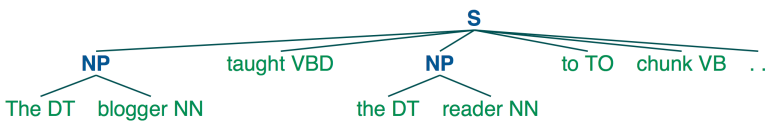
\includegraphics[width=\textwidth]{nickcdryanblog1.png}
    \caption{A sentence with simple NPs grouped}
\end{figure}\\
Let's try creating VPs now, the most simple grammar in this example would look like this:
\begin{verbatim}
    NP: {<DT>?<JJ>*<NN>} 
    VP: {<VBD>?<TO>?<VB>?}
\end{verbatim}
Run it through the algorithm above, and would you look at this:\\
\begin{figure}[htb!]
    \centering
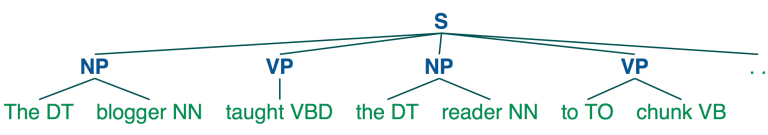
\includegraphics[width=\textwidth]{nickcdryanblog3.png}
    \caption{A sentence with simple NPs and VPs grouped}
\end{figure}\\
The issue with this grammar is that it works only with this one, simple approach proposed by the author of the blog. There are dozens of examples of custom NPs and VPs\cite{Constructing CFG} and it often turns out that the approaches are multiple-iterative and require a lot of computational complexity: \\ \\
\begin{figure}[htb!]
    \centering
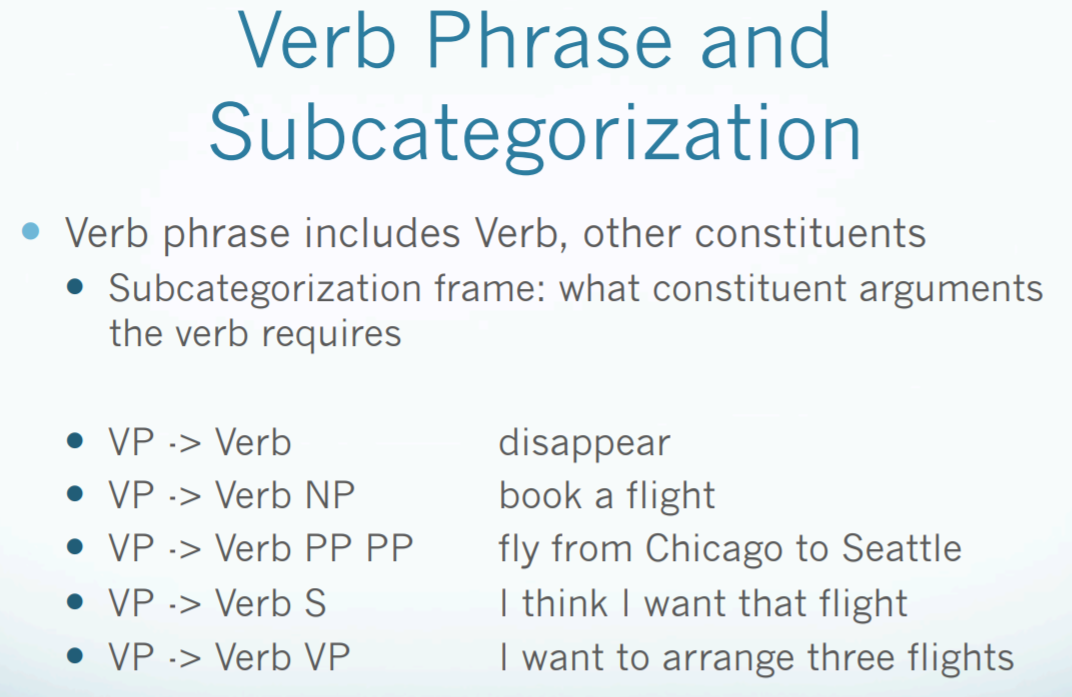
\includegraphics[width=\textwidth]{ProblemswithVPs.png}
    \caption{Some approaches at creating VP blocks}
\end{figure}

NLTK as a library supports multiple-attempt iterative approaches to grammars through the parameter "loop", where it is possible to create VPs out of VPs that did not exist on the first iteration.

\begin{verbatim}
    cp = nltk.RegexpParser(grammar, loop=2)
\end{verbatim}
Only on the second iteration the rule "VP $\rightarrow$ Verb VP" will be able to come into action, because on the first iteration no chunks were labeled as VPs to begin with. \\ \\
A few additional blocks can be derived using this approach, such as: Adjective Phrase (ADJP), Adverbial Phrase (ADVP) and Prepostional Phrase (PP)\cite{CFG for PP etc.}. All three of those can serve as potential checkpoints on the way to finding main NPs and VPs as seen in the figure below and they have their own creation rules just as well. \\ \\
\begin{figure}[htb!]
    \centering
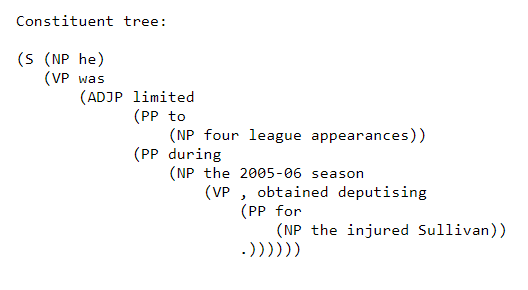
\includegraphics[width=0.6\textwidth]{NPsvsVPs.png}
    \caption{The main NP in this sentence that corresponds to the main VP is a "he". Because it is a PRP, one of the NP can be carried from the previous sentence.}
\end{figure}
\begin{figure}[htb!]
    \centering
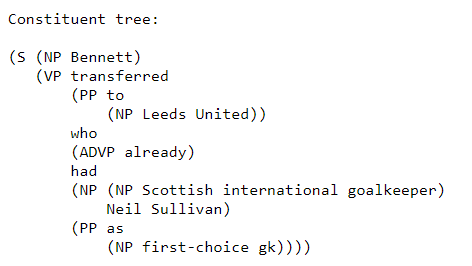
\includegraphics[width=0.6\textwidth]{NPsvsVPs2.png}
    \caption{The main NP in this sentence is "Benett", the actual agent of the sentence. Because "he" in the next sentence is a PRP, the NNP chunk of "Benett" can be carried over as the "he" of the next sentence.}
\end{figure}

Pronouns are always going to be located inside their own Noun Phrases and by looking over the influence of Verb Phrases on Noun Phrases, it is possible to prioritize certain Noun Phrases over the other when it comes to Pronouns. This approach is not always going to give perfect results, due to the fact that it's impossble to create a context-free grammar that would cover every sentence in the English Language. \\ \\
Consider the sentence "Long time no see", which has been adopted into English language, even though it is not entirely grammatically correct. It is still being used by people, even though the grammar tree of this sentence looks ambiguous.
\begin{verbatim}
    (S (VP (ADVP Long)
       time no see)
   .)
\end{verbatim}

\section{Machine Learning Challenges}
Because the chunks of text that are provided to us are multi-sentence, the most important challenge of this approach is to connect each pronoun (PRP) into the most significant named chunk (NNP) from the previous or the next sentence. \\ \\
Some sentences span for such a long time, that even tokenization into separate sentences will not do enough of the job and the sentences might need to be divided by "," signs just as well as "." signs. This creates its own set of problems, because, as shown in this very sentence, some comma-split sentences might span over a single word and by setting the agent tracking to just one sentence before a given sentence, the agent will be lost. \\ \\
Managing edge cases when a Context-Free grammar will not be able to return a clear answer on who is an agent in this sentence will require a more probabilistic approach. Distances between delimiters, NPs and VPs might be used to determine who the main agent is. \\ \\
More complex algorithms might require a lot of computational power, making the task assignment take too long to be feasible. \\ \\
Typos in sentences might lead to situations when NNPs will not be recognized as such and the PoS labels in NLTP will not return proper labels. Then, Machine Learning-based approach will have to improvise with the labels that it already has and try to readjust the sentence.
 
\begin{thebibliography}{9}
\bibitem{Tokenization}
\href{https://www.guru99.com/tokenize-words-sentences-nltk.html}{Tokenization in NLTP}

\bibitem{Demo of TweetTokenizer}
\href{https://stackoverflow.com/questions/37605710/tokenize-a-paragraph-into-sentence-and-then-into-words-in-nltk}{Code and demo on Stackoverflow}

\bibitem{POS}
\href{https://nickcdryan.com/2017/02/13/shallow-parsing-for-entity-recognition-with-nltk-and-machine-learning/}{More on PoS labels and chunking}

\bibitem{POS labels}
\href{https://medium.com/@gianpaul.r/tokenization-and-parts-of-speech-pos-tagging-in-pythons-nltk-library-2d30f70af13b}{List of all the PoS labels}

\bibitem{Constructing CFG}
\href{http://courses.washington.edu/ling571/ling571_WIN2015/slides/ling571_class2_grammar.pdf}{More on constructing Context-Free Grammars}

\bibitem{CFG for PP etc.}
\href{https://people.cs.umass.edu/~brenocon/inlp2017/lectures/16-cfg-exercise.pdf}{Context-free Grammars for VP, NP, PP, ADJP, ADVP and others.}
\end{thebibliography}
\end{document}
